\documentclass{beamer} 

% Michael Maier, 2013.
% CC-BY-SA

\usepackage[utf8]{inputenc}
\usepackage[ngerman]{babel}

\title{OpenStreetMap - Die freie Wiki-Weltkarte} 
\author{Michael Maier \textless Michael.Maier@student.tugraz.at\textgreater} 
\date{24. Oktober 2013} 

\usetheme{Antibes}

\hypersetup{colorlinks=true,urlcolor=blue,linkcolor=white}

%\usebackgroundtemplatei{
%
\includegraphics[width=\paperwidth,
%height=0.8\paperheight]{mag_map.png}
%}

\begin{document}

%\maketitle

\begin{frame} 


\begin{figure}
  \centering
  
\includegraphics[width=.5\textwidth]{mag_map.png}
\end{figure}

\begin{center}
\Huge{OpenStreetMap\\}
\end{center}

\begin{center}
\Large{\emph{Die freie Wiki-Weltkarte}}
\end{center}

\end{frame}



\begin{frame}{Vorstellung}

  \begin{itemize}
    \item Michael Maier \textless \href{mailto:Michael.Maier@student.tugraz.at}{Michael.Maier@student.tugraz.at}\textgreater
    \item Student an der TU Graz (Telematik)
    \item Linux-User (Debian/grml) seit 2004
      \begin{itemize}
                \item Organisiere Grazer Linuxtage seit 2011 mit
              \end{itemize}
    \item OpenStreetMap seit Juli 2010
    \item Leite den Grazer OSM-Stammtisch seit Mai 2011
    \begin{itemize}
      \item OSM-username: \emph{\href{http://www.openstreetmap.org/user/species}{species}}
      \item Mapping in Graz und auf Reisen mit Fahrrad und Öffis
    \end{itemize}
  \end{itemize}
\end{frame}

\section{Einleitung}

\begin{frame}{Was ist OpenStreetMap}

\begin{itemize}
  \item OpenStreetMap (OSM) ist eine freie Weltkarte nach dem Wiki-Prinzip „Wikipedia der Karten“
\pause
  \item Entsteht aus der Arbeit von \textgreater 1\,M Hobbykartografen „\emph{Mapper}“
\end{itemize}

 \begin{center}
 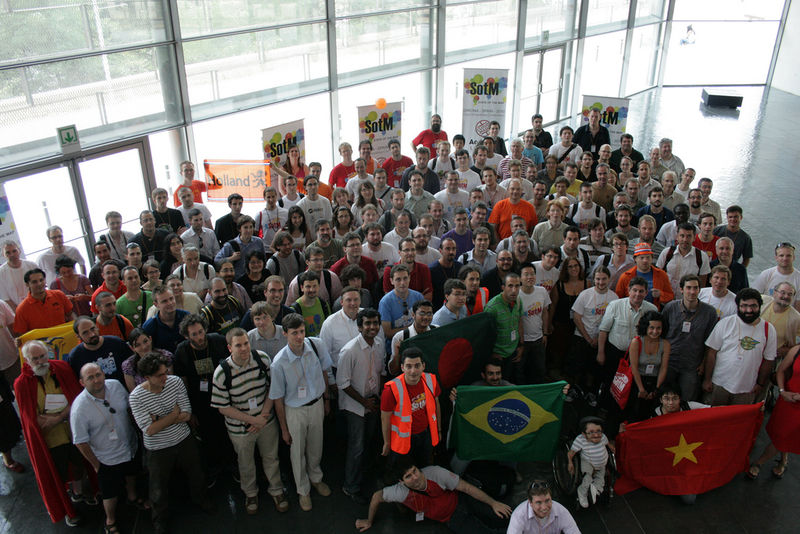
\includegraphics[width=5.5cm]{sotm.jpg}
 \end{center}

\end{frame}


\begin{frame}{Warum OpenStreetMap?}

Wir brauchen freie Karten!

\pause
\vspace{2mm}
Vorhandene Geodaten 
\begin{itemize}
  \item	für kommerzielle Nutzung zu teuer
  \item	wenn es sie denn gibt - zB Haiti
  \item	gratis nur für Lehre und Forschung
\end{itemize}

\pause
\vspace{2mm}
Karten kommerzieller Anbieter nur sehr restriktiv nutzbar
\begin{itemize}
  \item Restriktive Lizenzen - only Free as in Beer
  \item Offline-Nutzung oft nicht erlaubt - Roaming!
  \item Absichtliche Fehler, Änderungen/Richtigstellungen?
  \pause
  \item Bsp Google TOS: Durch die Nutzung schließen sie einen rechtsgültigen Vertrag mit Google - Dürfen unmündige Personen (unter 18?) Google Maps überhaupt nutzen?
  \item Kosten! Google verlangt ab 25K API-Zugriffen/Tag!
\end{itemize}

\end{frame}

\section{Wie funktioniert OpenStreetMap?}

\begin{frame}{Woher kommen unsere Daten?}

\begin{itemize}
  \item Freiwillige tragen ihr Wissen bei: Jeder weiß viel über seine Umgebung:
	\begin{itemize}
	  \item Hausnummern und Straßennamen,
	  \item Restaurants, Bars, POIs, ...
  \end{itemize}
  \pause
  \item Bei Mapping-Parties werden gezielt Gebiete verbessert...
\end{itemize}

 \begin{center}
 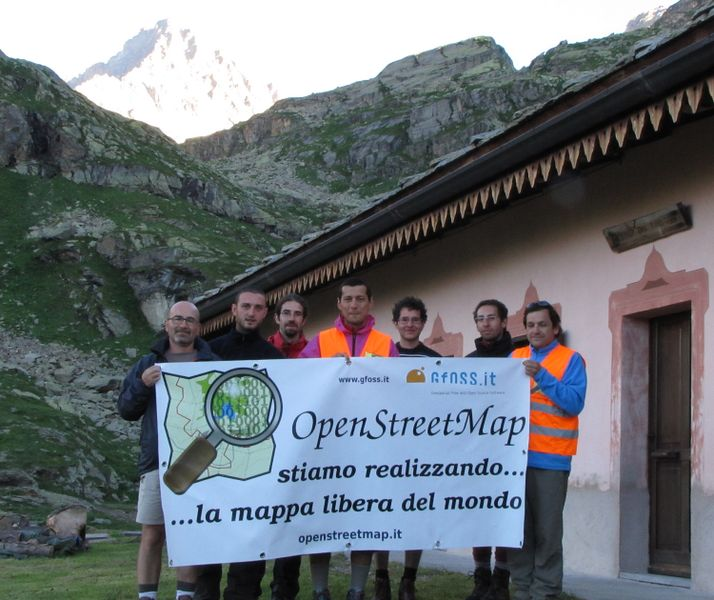
\includegraphics[width=5cm]{alps_mp.jpg}
 \end{center}

\end{frame}

\begin{frame}{Lizenz}

Die Daten stehen unter der Open Database Licence - Entspricht etwa Creative Commons - Attribution - Sharealike für Daten.
\begin{itemize}
  \item Jeder darf die Daten, auch kommerziell verwenden
  \item Quelle: „OpenStreetMap and Contributors, ODbL“ muß angegeben werden.
\end{itemize}

 \begin{center}
 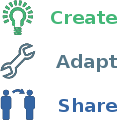
\includegraphics[width=1cm]{ODbL.png}
 \hspace{2cm}
 
\includegraphics[width=1.5cm]{cc-by-sa.png}
 \end{center}

\pause
Die Web-Karten auf \href{http://osm.org}{openstreetmap.org} sind CC-BY-SA.

\end{frame}

\section{Wie OpenStreetMap nutzen?}

\subsection{Interaktive Web-Karten}
\begin{frame}{ www.OpenStreetMap.org}

 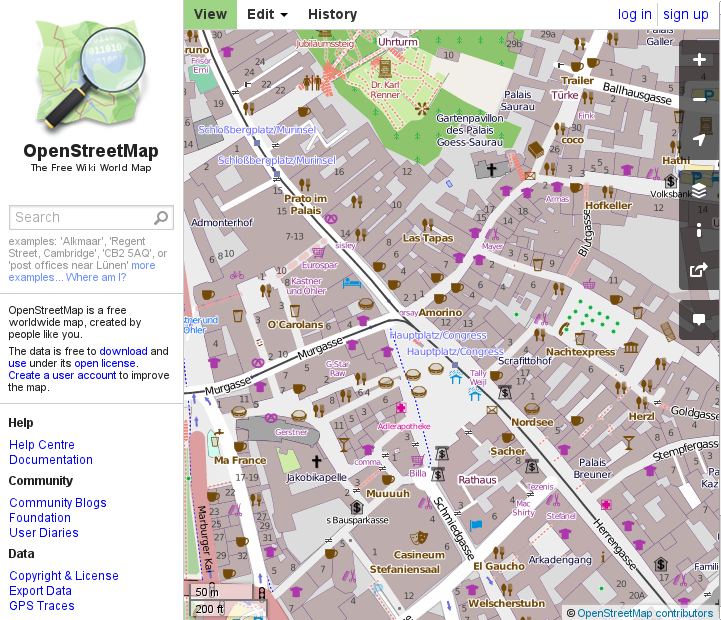
\includegraphics[width=11cm]{mainpage.png}

\end{frame}

\begin{frame}{ www.OpenStreetMap.org - Funktionen: Layer}

 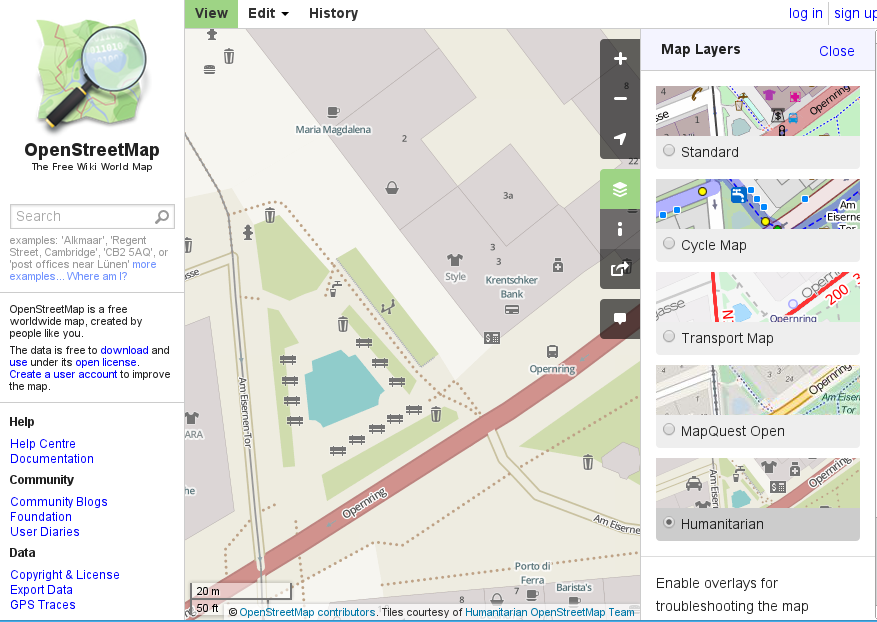
\includegraphics[width=11cm]{mainpage-layers.png}

\end{frame}

\begin{frame}{ www.OpenStreetMap.org - Funktionen: Notes}

 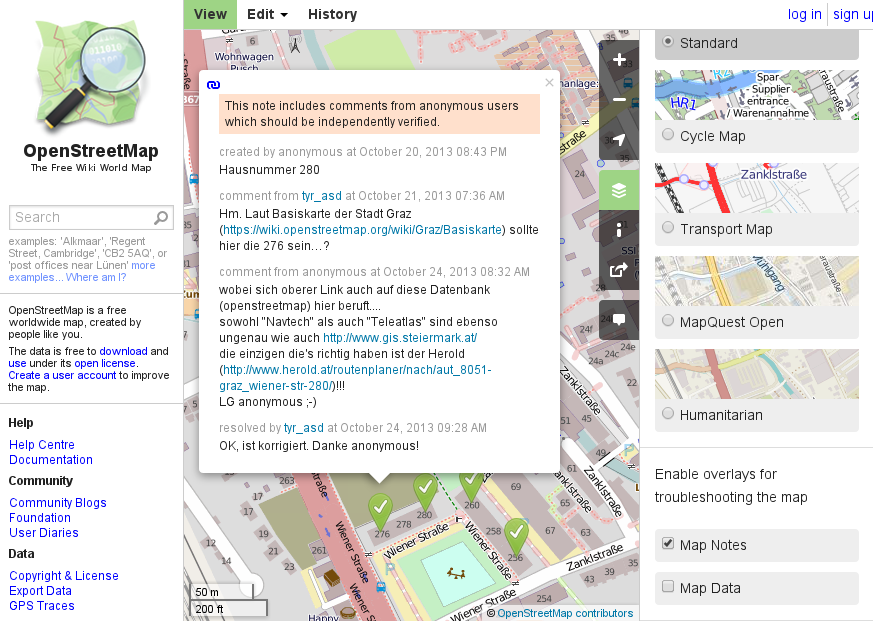
\includegraphics[width=10cm]{mainpage-notes.png}

\end{frame}

\begin{frame}{ www.OpenStreetMap.org - Funktionen: Daten ansehen}

 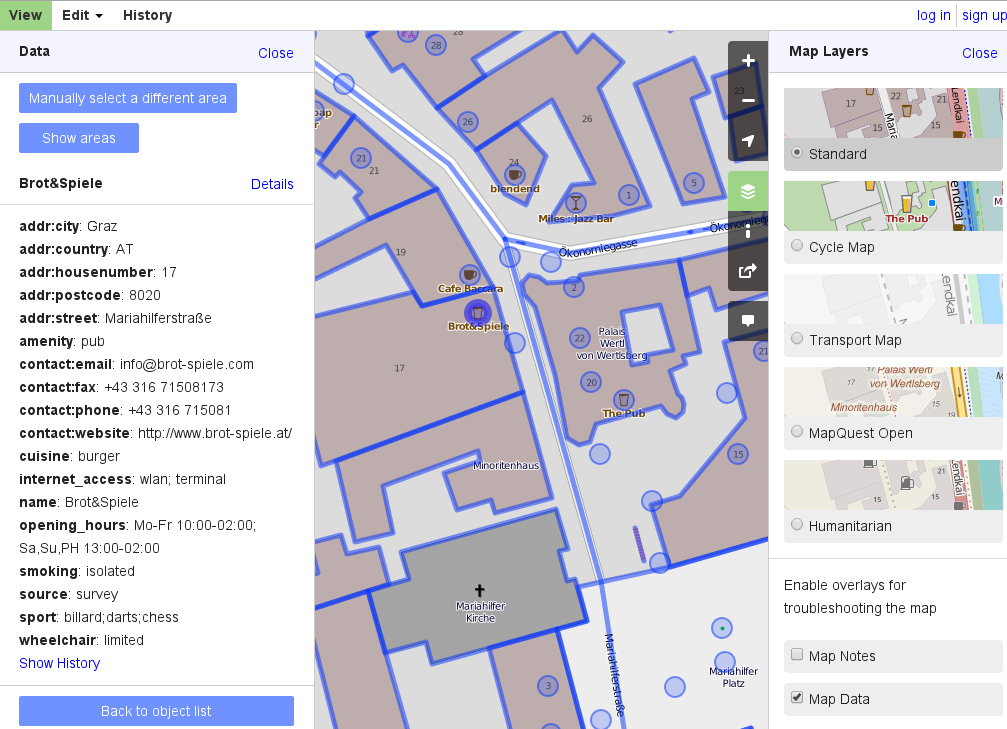
\includegraphics[width=10cm]{mainpage-data.png}

\end{frame}

\begin{frame}{Spezialkarten:}


  \begin{table}[htbp]
    \centering
    \begin{tabular}{r|l}
      Radkarte  &  \url{http://opencyclemap.org} \\
      Wanderkarte & \url{http://hikebikemap.de} \\
      Rauchfrei-Karte & \url{http://OpenGastroMap.org} \\
      Rollstuhl-Karte & \url{http://wheelmap.org} \\
      Seekarte & \url{http://OpenSeaMap.org} \\
\pause
      200 weitere: & siehe \href{http://wiki.openstreetmap.org/wiki/List\_of\_OSM\_based\_Services}{OSM-Wiki} \\
%      Interaktive Informationskarte & http://openstreetbrowser.org
    \end{tabular}
  \end{table}

  Blitzschnelles Routing: \url{http://osrm.at} \hspace{1cm} 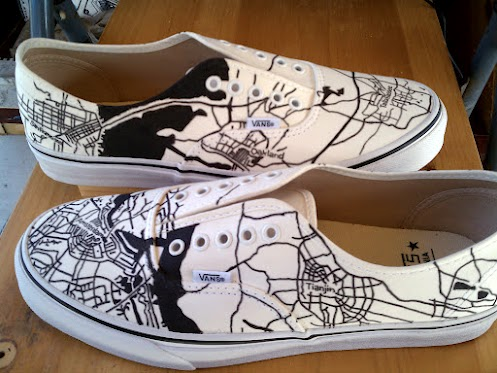
\includegraphics[width=2.5cm]{shoes.jpg}

\end{frame}

\subsection{Mobil}
\begin{frame}{Aus Smartphones/Tablets nutzen:}
	Apps:
 
 \begin{itemize}
   \item  Android ( \textgreater 70) \url{http://wiki.osm.org/Android}
   \item  iPhone ( \textgreater 60 )  \url{http://wiki.osm.org/Apple\_iOS}
   \item  Blackberry ( 8 ) \url{http://wiki.osm.org/BlackBerry\_OS}
 \end{itemize}
 
 \begin{center}
 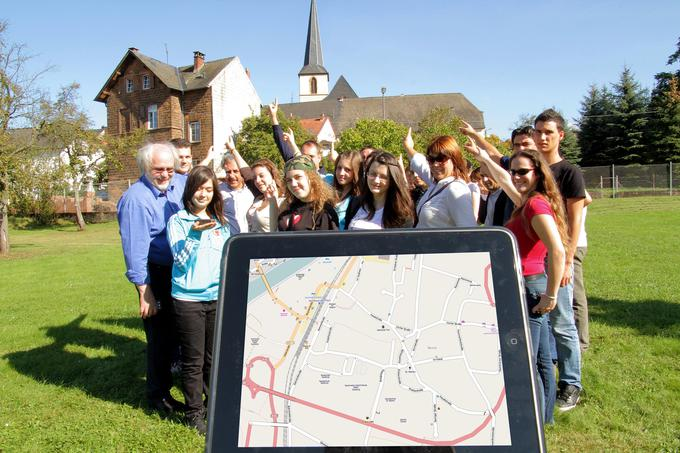
\includegraphics[width=5cm]{tablet.jpg}
 \end{center}

 Natürlich auch auf Navis, am OSM-freundlichsten sind Garmin: \href{http://wiki.osm.org/Garmin}{wiki.osm.org/Garmin}!

\end{frame}

  \subsection{ OpenStreetMap Verbessern}

\begin{frame}{OpenStreetMap Verbessern}

  Eine große Auswahl an Editoren steht fürs Web, Desktop- und Mobilnutzung zur Verfügung

  \begin{itemize}
    \item Web:
    \begin{itemize}
	    \item Hauptseite - Edit: iD (JavaScript)
      \item JOSM web-start
      \item oder auch einfach nur Fehler melden!
	      \pause
    \end{itemize}
    \item Mobile (Auswahl): Alle siehe  \href{http://wiki.openstreetmap.org/wiki/Android\#OpenStreetMap\_editing\_features}{Android}, \href{http://wiki.openstreetmap.org/wiki/Apple\_iOS\#OpenStreetMap\_editing\_features}{iOS}:
    \begin{itemize}
      \item Vespucci: Ausgewachsener Editor
      \item osmaptuner: Existierende POIs ergänzen
      \item OsmTracker: GPS-Tracks, Audio, schnell POIs hinzufügen
    \end{itemize}
  \item Desktop
    \begin{itemize}
      \item \href{http://josm.openstreetmap.de}{JOSM}
      \item \href{http://merkaartor.be}{Merkaartor}
    \end{itemize}
  \end{itemize}

\end{frame}

\begin{frame}{Die Zukunft... 3D! }
  Neu! Jetzt auch in 3D! Beispielsweise auf \href{http://maps.osm2world.org/?zoom=17&lat=47.06156&lon=15.46983&layers=BF0FTFFF}{maps.osm2world.org}.

  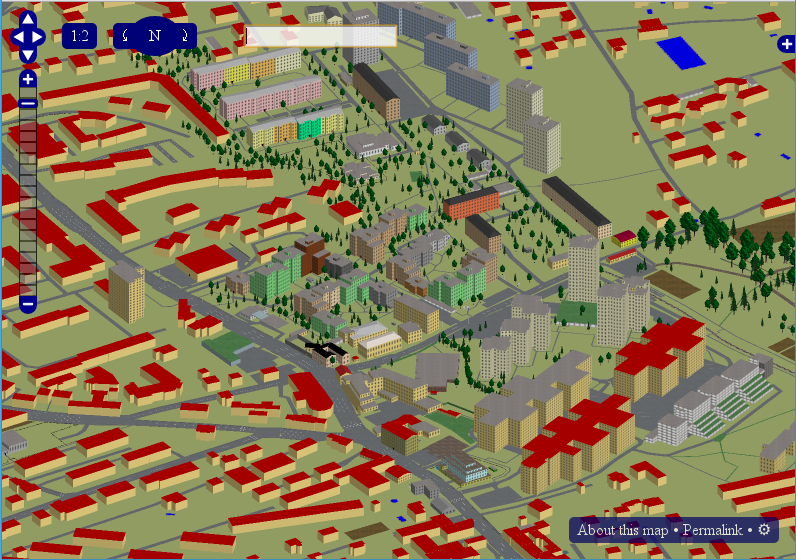
\includegraphics[width=0.9\textwidth]{3d.png}


\end{frame}

\begin{frame}{Hilfe}

\begin{itemize}
  \item Fragen? Heute oder morgen durchgehend!
\end{itemize}
 \begin{center}
	  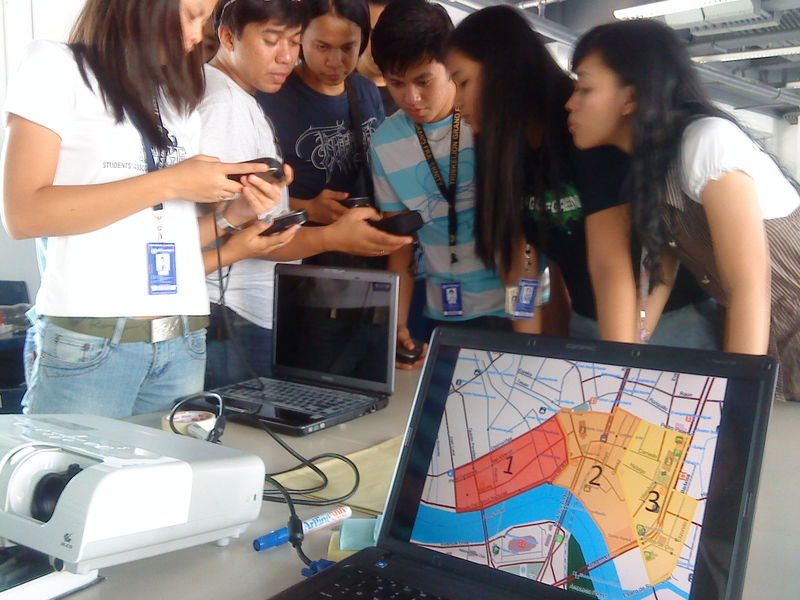
\includegraphics[width=4cm]{osm_workshop.jpg}
 \end{center}
\begin{itemize}
  \item Informationen: Wiki \href{http://wiki.openstreetmap.org}{wiki.openstreetmap.org}
  \item Immer noch etwas unklar? $\Rightarrow$ Mailingliste \href{http://lists.openstreetmap.org/listinfo/talk-at}{talk-at}
  \pause
  \item \href{http://wiki.openstreetmap.org/wiki/Graz/Stammtisch}{Stammtisch Graz} jedes Monat - der nächste Montag, 16.11.2013, Brot und Spiele!
\end{itemize}

\end{frame}

\section{Ende}

\begin{frame}{Vielen Dank für die Aufmerksamkeit!}

  Folien zu „Graz, offene Stadt?“ am Elevate 2013, Graz
\vspace{1cm}

Folien unter: 
\includegraphics[width=1cm]{cc-by-sa.png}.
\vspace{1cm}

Erstellt mittels \LaTeX Beamer, Quelltext: \url{https://github.com/species/vortrag-osm-elevate13}.
\vspace{1cm}

\href{mailto:michael.maier@student.tugraz.at}{Michael Maier}

Twitter: \href{https://twitter.com/osmgraz}{@osmgraz}
\end{frame}

\end{document}
